%!TeX root = ../main.tex


\section{Conclusions}
By performing a reconstruction in COLMAP, a final result is obtained and in this case, as shown in fig. \ref{fig:fountainautoenc} and \ref{fig:tisoautoenc}, the fountain and the building are rebuilt in a more sparse form due to the smaller amount of information provided to the software. Fig. \ref{fig:fountaintrue} and \ref{fig:tisotrue} refer to the final result without the use of the autoencoder and therefore all the features and matchings obtained by the SURF algorithm are supplied to COLMAP without regression. Comparing the two results, significant differences are visible in the reconstruction quality of the subjects.


\begin{figure}[H]
     \centering
     \begin{subfigure}[b]{0.48\textwidth}
		\centering
		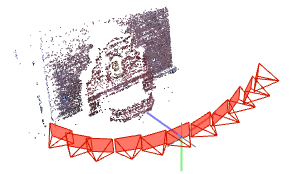
\includegraphics[width=\textwidth]{images/fountainautoenc.png}  
		\caption{\centering Fountain reconstructed with the autoencoder.}
	    	\label{fig:fountainautoenc} 
     \end{subfigure}
     \hfill
     \begin{subfigure}[b]{0.48\textwidth}
		\centering
    		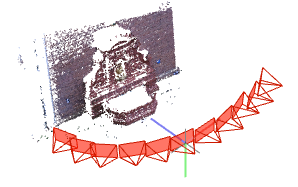
\includegraphics[width=\textwidth]{images/fountaintrue.png}
		\caption{\centering Fountain reconstructed without the autoencoder.}
		\label{fig:fountaintrue}   
     \end{subfigure}
        \caption{Fountain reconstruction using COLMAP.}
        \label{fig:Fountain3D}
\end{figure}


\begin{figure}[H]
     \centering
          \begin{subfigure}[b]{0.48\textwidth}
		\centering
    		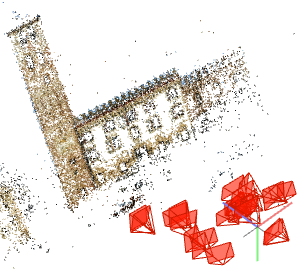
\includegraphics[width=\textwidth]{images/tisoautoenc.png}
		\caption{\centering Tiso reconstructed with the autoencoder.}
		\label{fig:tisoautoenc}   
     \end{subfigure}
     \hfill
     \begin{subfigure}[b]{.48\textwidth}
		\centering
		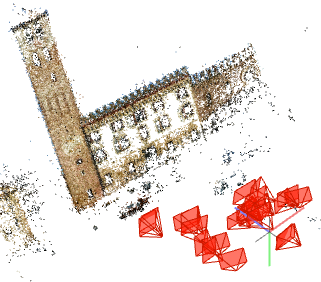
\includegraphics[width=\textwidth]{images/tisotrue.png}  
		\caption{\centering Tiso reconstructed without the autoencoder.}
	    	\label{fig:tisotrue} 
     \end{subfigure}
        \caption{Tiso reconstruction using COLMAP.}
        \label{fig:Tiso3D}
\end{figure}

From the parameters obtained after the reconstruction, reported in the table \ref{table:result} regarding the Fountain-P11 dataset, there is a mean observations per image equal to 4751.36 and a total number of observations equal to 52256, in the case of the compression strategy. Data are almost a third lower than those obtained with the SURF algorithm without using the autoencoder. Also the other parameters have substantial differences such as the number of points that is half between the compared data.

\begin{table}[h!]
\centering
\begin{tabular}{ |c|c|c| } 
\hline
\textbf{Parameters} & \textbf{No autoencoder} & \textbf{Autoencoder} \\ [0.5ex]
\hline
 Cameras & 11 & 11 \\ [0.5ex]
 Images & 11 & 11 \\ [0.5ex]
 Points & 30620 & 14674 \\ [0.5ex]
 Observations & 139909 & 52265 \\ [0.5ex]
 Mean track length & 4.5692 & 3.56174 \\ [0.5ex]
 Mean observations per image & 12791 & 4751.36 \\ [0.5ex]
 Mean reprojection error & 0.49785 & 0.428602 \\ [0.5ex]
 \hline
\end{tabular}
 \caption{\centering Result comparisons for Fountain-P11 between the no-autoencoder and autoencoder strategies.}
 \label{table:result}
\end{table}

Fig. \ref{fig:matrix} reports the difference between the match matrices in the case of regression or not and displays a qualitative measure of the matchings in the reconstruction process in COLMAP. Figure \ref{fig:matrixautoenc} displays a smaller variance, i.e. a smaller number of matchings per feature, due to the compression.

\begin{figure}[H]
     \centering
          \begin{subfigure}[b]{0.40\textwidth}
		\centering
    		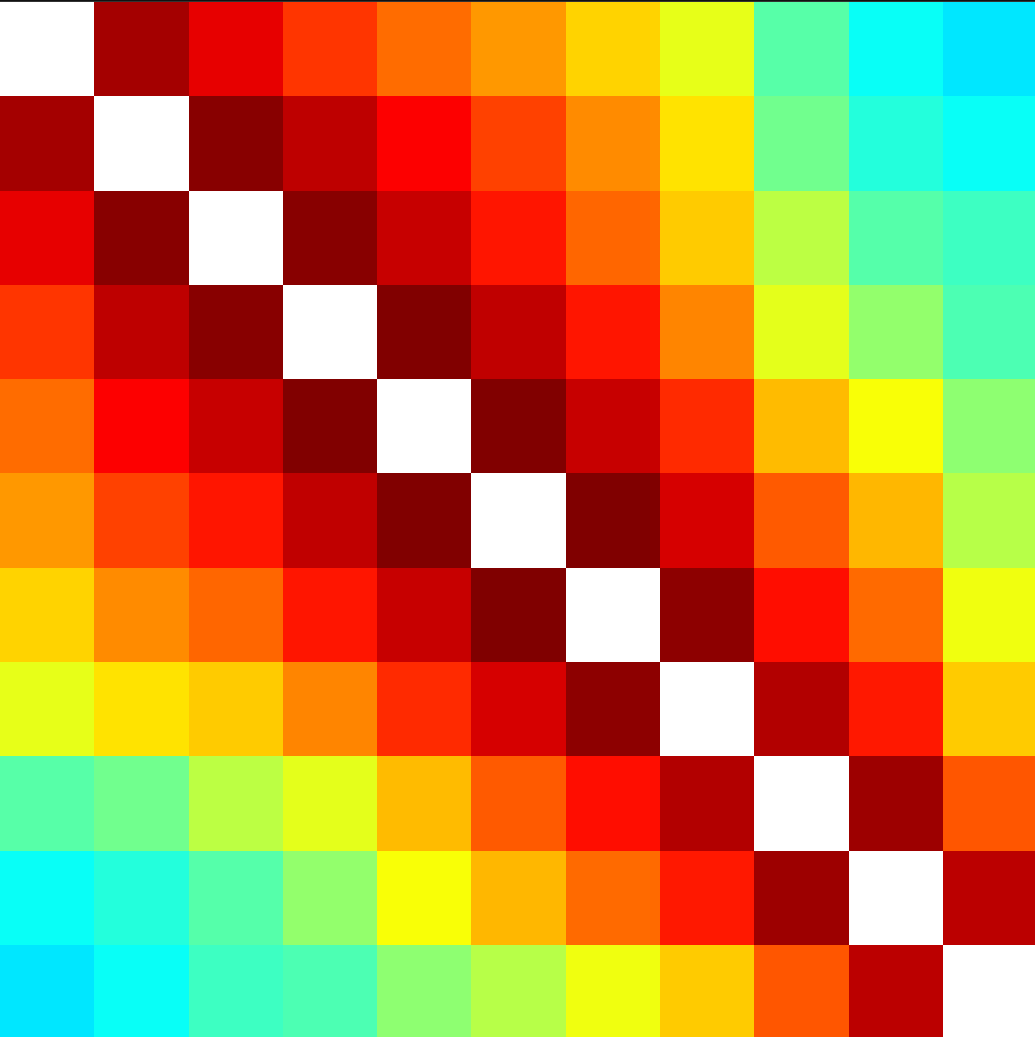
\includegraphics[width=\textwidth]{images/matrix.png}
		\caption{\centering Match matrix without the autoencoder.}
		\label{fig:matrix1}   
     \end{subfigure}
     \hfill
     \begin{subfigure}[b]{.40\textwidth}
		\centering
		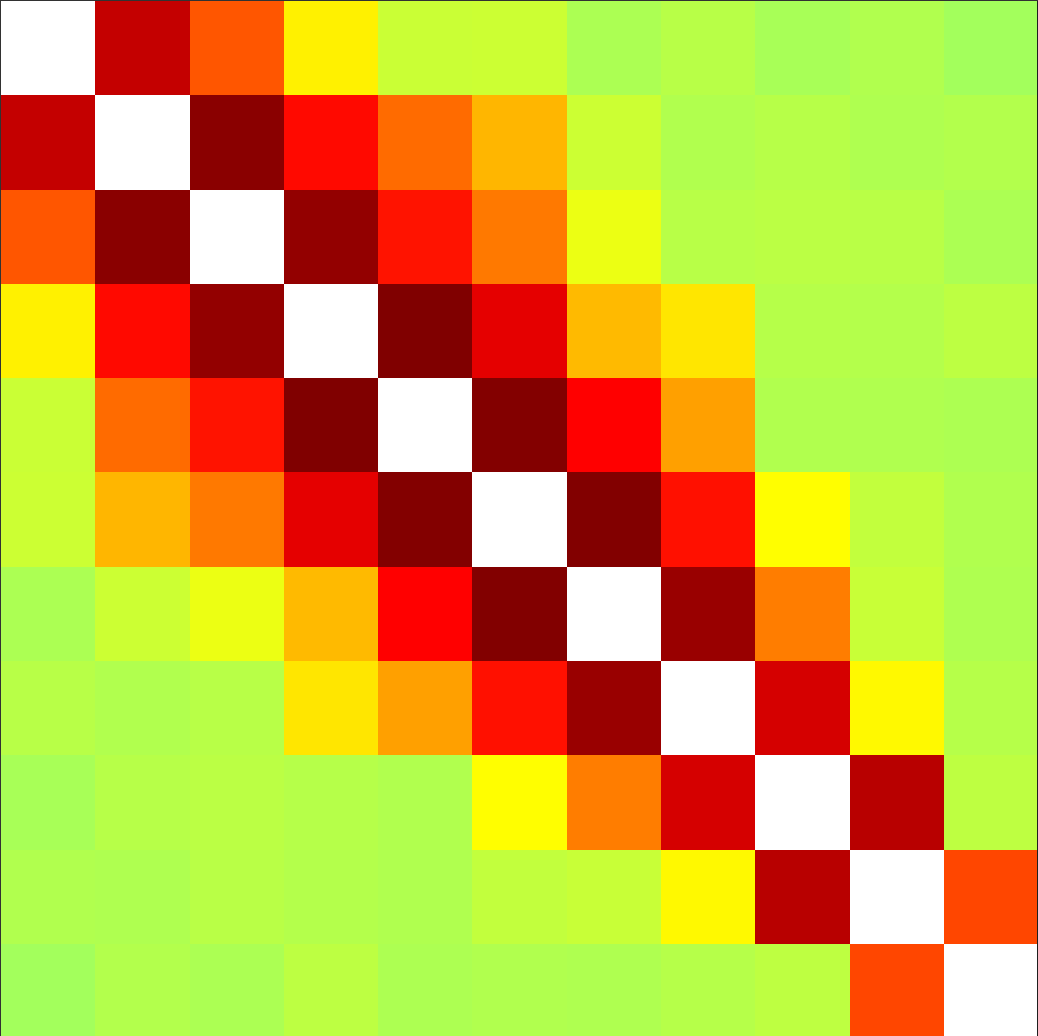
\includegraphics[width=\textwidth]{images/matrixautoenc.png}  
		\caption{\centering Match matrix with the autoencoder.}
	    	\label{fig:matrixautoenc} 
     \end{subfigure}
        \caption{Match matrix comparison.}
        \label{fig:matrix}
\end{figure}

This type of strategy is surely a \emph{lossy} compression, which sacrifices part of the original information during the decompression phase of the data in order to reduce the computational complexity and/or the original dimensions. It can be useful in environments where the quality of reconstruction is not important, for example in object detection, where is not crucial to exactly reconstruct the object with respect to the detection result ``true/false''. It can be seen from the compressed images that the edges of the objects are mostly preserved while straight planes are ``thinned out'', i.e. represented with less points. This means that the most important part of the original information (larger variance) is preserved and classifies the autoencoder compression strategy as a useful tool in many appliable fields.